\section{Fourier Series}

So far we've considered initial value problems while solving ODEs. While looking at second-order ODEs, we are given the value of the function and its derivative at a given time. In boundary value problems, we are given the value of the function at two different points (i.e. 2 points on the boundary of the domain).

Boundary eigenvalue problems are a generalisation to functions of eigenvalue problems for matrices. This yields eigenvectors that form a basis in a function space. 

\subsection{Boundary Value \& Eigenvalue Problems}\label{sec:boundaryvalprob}

\begin{eg}\label{eg:bvpmotiv}
	We consider the following boundary value problem involving a second-order ODE:
	\[
	y'' + y = 0 \qquad y'(0)=1, \,\, y(\pi) = a
	\]
	
	The solution is given by: 
	\[
	y = A \cos{x} + B \sin{x}
	\]
	Imposing the boundary conditions:
	\begin{align*}
		y(0) &= A = 1 \\
		y(\pi) &= -A = a
	\end{align*}
	
	If $a \neq -1$, then there is no solution to the boundary value problem.
	
	If $a = -1$, there are infinitely many solutions to the boundary value problem as $y(x) = \cos{x} + B\sin{x}$ where $B \in \R$. 
\end{eg}
	
This illustrates one way in which boundary value problems differ from initial value problems: while the IVP
\[
	y'' + p(t)y' + q(t)y = g(t), \quad y(t_0) = \alpha, y'(t_0) = \beta
\]
is guaranteed to have a unique solution on an open interval $I$ provided that $p$, $q$, and $g$ are continuous on $I$, the boundary value problem
\[
	y'' + p(x)y' + q(x)y = g(x), \quad y(x_1) = \alpha, y(x_2) = \beta
\]
could have a unique solution, many solutions, or no solution, depending on the boundary conditions.
	
The above \Cref{eg:bvpmotiv} having infinitely many solutions in the case of $a = -1$ is similar to the case of $A\vbx = \bm{b}$ where $A$ is a singular matrix. There are no solutions to this system unless $\bm{b}$ is orthogonal to any vector in the kernel of $A^T$. So, $\bm{b} \cdot \bm{y} = 0$ for all $\bm{y} \in \R^n$ such that $A^T \bm{y} = 0$.

Recall the matrix eigenvalue problem: 
\begin{equation}\label{eq4.1}
	A \xib_i = \lambda_i \xib_i
\end{equation}
The eigenvalue problem helps us find non-trivial solutions to \Cref{eq4.1}, which will exist only if $\lambda_i$ are eigenvalues of $A$. In addition, if $A$ is diagonalisable, then $\xib_i$ form a basis of $\R^n$ and $\xt = \sum_{i=1}^n c_i \xib_i$.

If $A^T = A$, the matrix is symmetric and the eigenvectors are orthogonal so $\xib_i \cdot \xib_j = 0$ for $i \neq j$. So, we have that
\begin{align*}
	\vbx &= \sum_{i=1}^n c_i \xib_i \\
	\xib_j \cdot \vbx &= \sum_{i=1}^n c_i \xib_i \cdot \xib_j
\end{align*}
but since $\xib_i \cdot \xib_j = 0$ for $i \neq j$, 
\begin{align*}
	\xib_j \cdot \vbx = c_j \Vert \xib_j \Vert^2
\end{align*}
So, in this case, the fact that the basis is orthogonal makes finding the coefficients $c_i$ easier when we want to represent some vector using this basis.


We now look at an equivalent of the eigenvalue problem $A \xib = \lambda \xib$. We can consider $A$ to be a linear map and we know that linear maps can act on functions. An operator $Ly(x)$ is linear if and only if $L(ay_1(x) + by_2(x)) = aLy_1(x) + bLy_2(x)$

\begin{eg}\label{eg:linearmap}
	The following are linear operators:
	\begin{itemize}
		\item $L = \frac{d^2}{dx^2}$ since $\frac{d^2}{dx^2}(ay_1 + by_2) = a \frac{d^2}{dx^2}y_1 + b \frac{d^2}{dx^2}y_2$.
		\item $L = p(x)\frac{d^2}{dx^2} + q(x)\frac{d^2}{dx^2}$.
	\end{itemize}
\end{eg}

So the generalisation of eigenvalue problems for functions would be $Ly(x) = \lambda y(x)$.

\begin{eg}\label{eg:eigenvalprob}
	\[
	y'' = \lambda y \qquad y(0) = y(L) = 0
	\]
	We look at the following 3 cases:
	\begin{itemize}
		\item Case 1: $\lambda = \mu^2 > 0$.\\
		The ODE is given by: $y'' - \mu^2 y = 0$.\\
		In this case, the solution is given by:\footnote{Since $e^{\mu x}$ and $e^{-\mu x}$ are fundamental solutions, and $\cosh{\mu x} = \frac12(e^{\mu x} + e^{-\mu x})$ and $\sinh{\mu x} = \frac12(e^{\mu x} - e^{-\mu x})$ i.e. they are linear combinations of $e^{\mu x}$ and $e^{-\mu x}$.}
		\[
		y(x) = A \cosh{\mu x} + B \sinh{\mu x}.
		\]
		Using the boundary values:
		\begin{align*}
			y(0) &= A = 0 \\
			y(L) &= B \sinh{\mu L} = 0 \implies B=0
		\end{align*}
		So there is no non-trivial solution in this case.
		
		\item Case 2: $\lambda = 0$.\\
		The ODE is given by: $y''= 0$.\\
		In this case, the solution is given by:
		\[
		y(x) = Ax + B.
		\]
		Using the boundary values:
		\begin{align*}
			y(0) &= B = 0 \\
			y(L) &= AL = 0 \implies A = 0
		\end{align*}
		So there is no non-trivial solution in this case.
		
		\item Case 3: $\lambda = -\mu^2 < 0$.\\
		The ODE is given by: $y'' + \mu^2 y = 0$.\\
		In this case, the solution is given by:
		\[
		y(x) = A \cos{\mu x} + B \sin{\mu x}.
		\]
		Using the boundary values:
		\begin{align*}
			y(0) &= A = 0 \\
			y(L) &= B \sin{\mu L} = 0
		\end{align*}
		In this case, however, $B \neq 0$ if $\mu L = n \pi$ where $n \in \Z$. So, we have non-trivial solutions $\lambda = -\mu^2$ where $\mu = \frac{n \pi}{L}$.
	\end{itemize}
	Thus, the eigenvalues are given by: $\lambda_n = -\frac{n^2\pi^2}{L^2}$, where $n = 1, 2, \dots$, and the eigenfunctions are given by: $y_n(x) = \sin\left(\frac{n\pi x}{L}\right)$.
	
	So, we have a set of eigenvalues and eigenfunctions for the ODE.
\end{eg}

\begin{eg}\label{eg:bvpmotiv2}
	\[
	y'' = \lambda y \qquad y(x+2L) = y(x)
	\]
	Here, we see a periodic function with period $2L$. Equivalently,
	\begin{align*}
		y(-L) &= y(L) \\
		y'(-L) &= y'(L)
	\end{align*}
	\begin{itemize}
		\item Case 1: $\lambda = \mu^2 > 0$.\\
		The ODE is given by: $y'' - \mu^2 y = 0$.\\
		In this case, the solution is given by:
		\[
		y(x) = A \cosh{\mu x} + B \sinh{\mu x},
		\]
		Using the boundary conditions:
		\begin{align*}
			y(-L) &= A \cosh{\mu L} - B \sinh{\mu L} \\
			y(L) &= A \cosh{\mu L} + B \sinh{\mu L} \\
			y(-L) &= y(L) \implies B = 0 \\
			y'(-L) &= y'(L) \implies A = 0 
		\end{align*}
		So, there is no non-trivial solution in this case.
		
		\item Case 2: $\lambda = 0$.\\
		The ODE is given by: $y''= 0$.\\
		In this case, the solution is given by:
		\[
		y(x) = Ax + B.
		\]
		Using the boundary conditions:
		\begin{align*}
			y(-L) &= -AL + B\\
			y(L) &= AL + B \\
			y(-L) &= y(L) \implies A = 0 \\
			y'(-L) &= y(L) \implies B \text{ is a free parameter.}
		\end{align*}
		So, the only non-trivial function in this case is the constant function $y(x)=B$.
		
		\item Case 3: $\lambda = -\mu^2 < 0$.\\
		The ODE is given by: $y'' + \mu^2 y = 0$.\\
		In this case, the solution is given by:
		\[
		y(x) = A \cos{\mu x} + B \sin{\mu x}
		\]
		Using the boundary conditions:
		\begin{align*}
			y(-L) & = A \cos{\mu L} - B \sin{\mu L} \\
			y(L) & = A \cos{\mu L} + B \sin{\mu L}
		\end{align*}
		\[
		y(-L) = y(L) \implies B \sin{\mu L} = 0 \implies \mu L = n \pi
		\]
		\begin{align*}
			y'(-L) & = \mu A \sin{\mu L} + \mu B \cos{\mu L} \\
			y'(L) & = -\mu A \sin{\mu L} + \mu B \cos{\mu L}
		\end{align*}
		\[
		y'(-L) = y'(L) \implies A \sin{\mu L} = 0 \implies \mu L = n \pi
		\]
		So, we have non-trivial solutions $\lambda = -\mu^2$ where $\mu = \frac{n \pi}{L}$.
	\end{itemize}
	Thus, the eigenvalues are given by: $\lambda_n = -\frac{n^2\pi^2}{L^2}$, where $n =0, 1, 2, \dots$, and the eigenfunctions are given by: $1, \cos\left(\frac{n\pi x}{L}\right), \sin\left(\frac{n\pi x}{L}\right)$.
	
	So, we have found a set of eigenvalues and eigenfunctions for the ODE.
\end{eg}

\subsection{Euler-Fourier Formulas}

\begin{definition}
	A function $f(x)$ is periodic if $f(x+T) = f(x) \,\, \forall x$. We say its	period is $T$. The smallest possible $T$ is the \textbf{fundamental period}.
\end{definition}

\begin{remark}
	Note that the convention used here is that that the period is $2L$, as is also used by Boyce. Other texts may differ, however.
\end{remark}

The Fourier series is a series that expresses a periodic function as an infinite sum of sines and cosines.
\begin{definition}\label{def:fourier}
	The Fourier series for a function $f(x)$ with period $2L$ is given by: 
	\[
		f(x) = \frac{a_0}{2} + \sum_{n=1}^{\infty} \left(a_n \cos{\left(\frac{n\pi x}{L}\right)} + b_n \sin{\left(\frac{n\pi x}{L}\right)}\right)
	\]
	where $a_0, a_n, b_n$ are coefficients that can be calculated using the Euler-Fourier formulas. The coefficients are real if $f(x)$ is real.
\end{definition}

Considering periodic functions $f(x+2L) = f(x)$, we looked at the eigenvalue problem: $y'' = \lambda y$ in \Cref{eg:bvpmotiv2}. The eigenvalues were found to be
\[
\lambda_n = -\frac{n^2 \pi^2}{L^2} 
\]
and corresponding eigenfunctions were 
\begin{align*}
	n &= 0, \quad y_0 = 1 \\
	n &\neq 0, \quad y_n = \cos{\left(\frac{n \pi x}{L}\right)}, \sin{\left(\frac{n \pi x}{L}\right)}
\end{align*}
So the basis is given by: $\left\{1, \cos{(\frac{n \pi x}{L})}, \sin{(\frac{n \pi x}{L})}\right\}$.

It is useful to have that the eigenfunctions are orthogonal. In this case, consider the inner product (the dot product) given by:
\begin{equation}\label{eq:innerprod}
	(u(x), v(x)) = \int_{-L}^L u(x) v(x) dx
\end{equation}
Then , the functions $\{1, \cos{(\frac{n \pi x}{L})}, \sin{(\frac{n \pi x}{L})}\}$ are orthogonal for this inner product.

The proof is as follows: Denote $C_n(x) = \cos{(\frac{n \pi x}{L})}$, $S_n(x) = \sin{(\frac{n \pi x}{L})}$, and $C_0(x)=1$. Now, consider
\begin{align*}
	\left(S_n(x), S_m(x)\right) &= \int_{-L}^L \sin{\left(\frac{n \pi x}{L}\right)} \sin{\left(\frac{m \pi x}{L}\right)} \,dx \\
	&= \frac{1}{2} \int_{-L}^L \cos{\left(\frac{(n-m) \pi x}{L}\right)} - \cos{\left(\frac{(n+m) \pi x}{L}\right)} \,dx
\end{align*}
If $n \neq m$, then
\[
\left(S_n(x), S_m(x)\right) = \frac{L}{2} \left(  \begin{bmatrix}\dfrac{\sin{\left(\frac{(n-m) \pi x}{L} \right)} }{(n-m) \pi} \end{bmatrix}_{-L}^L - \ \begin{bmatrix} \dfrac{\sin{\left(\frac{(n+m) \pi x}{L} \right)} }{(n+m) \pi} \end{bmatrix}_{-L}^L \right) = 0,
\]
since at every point we are evaluating sin at some integer multiple of $\pi$, which is zero.

If $n = m$, then
\begin{align*}
	\left(S_n(x), S_n(x)\right) & = \int^L_{-L} \sin^2{\left(\frac{n \pi x}{L}\right)} dx = \frac{1}{2} \int^L_{-L} 1 - \cos{\left(\frac{n \pi x}{L}\right)} dx \\
	&= \frac{1}{2}\left( 2L - L \left[ \sin{\left(\frac{2 \pi x}{L} \right)} \right]_{-L}^L \right) = L.
\end{align*}
From the above, we see that the sin functions have orthogonality as:
\[
(S_n, S_m) = L \delta_{mn} \quad \text{where } \delta_{mn} = \begin{cases}0 & \text{if } m \neq n \\ 1 & \text{if } m = n
\end{cases}
\]
where $\delta_{mn}$ is the Kronecker delta.

Similarly, we find that:
\[
(C_n, C_m) = L \delta_{mn} \quad \text{where } \delta_{mn} = \begin{cases}0 & \text{if } m \neq n \\ 1 & \text{if } m = n
\end{cases}
\]
And finally,
\begin{align*}
	(S_n, C_m) &= 0 \\
	(C_0, C_0) &= 2L
\end{align*}
The calculations of these two are left as an exercise to the reader.

With this information in hand, we are now ready to find the Fourier series for a $2L$ periodic function $f$. Reminder from \Cref{def:fourier} that the Fourier series is
\[
f(x) = \frac{a_0}{2} + \sum_{n=1}^{\infty} \left(a_n \cos{\left(\frac{n\pi x}{L}\right)} + b_n \sin{\left(\frac{n\pi x}{L}\right)}\right)
\]
where $a_n, b_n$ are Fourier coefficients. The coefficient of function $C_0 = 1$ is $\frac{a_0}{2}$.

To calculate $a_n, b_n$, we project $f(x)$ on the basis as follows (for $n \neq 0$): 
\begin{align*}
	(f(x), C_n) & = \left( \frac{a_0}{2} + \sum_{m=1}^{\infty} \left(a_m C_m(x) + b_m S_m(x) \right), C_n \right) \\
	& = \frac{a_0}{2}\cancelto{0}{(1,C_n)} + \sum_{m=1}^{\infty} a_m\cancelto{L\delta_{mn}}{(C_m, C_n)} + \sum_{m=1}^{\infty} b_m\cancelto{0}{(S_m, C_n)} \\
	&= a_n L.
\end{align*}

Therefore,
\begin{align*}
	a_n = \frac{1}{L} (f(x), C_n(x)) = \frac{1}{L} \int_{-L}^L f(x) \cos{\left(\frac{n \pi x}{L}\right)} dx
\end{align*}\

Similarly, $b_n$ is calculated by projecting $f$ on $\sin{\left( \frac{n \pi x}{L} \right)}$ and using orthogonality we get:
\[
b_n = \frac{1}{L} \int_{-L}^L f(x) \sin{\left( \frac{n \pi x}{L} \right)} dx
\]

Thus, we have the Euler-Fourier formulas:
\begin{align}
	\label{eq:eulerfourier1}
	a_n &= \frac{1}{L} \int_{-L}^L f(x) \cos{\left( \frac{n \pi x}{L} \right)} dx \\
	\label{eq:eulerfourier2}
	b_n &= \frac{1}{L} \int_{-L}^L f(x) \sin{\left( \frac{n \pi x}{L} \right)} dx \\
	\label{eq:eulerfourier3}
	a_0 &= \frac{1}{L} \int_{-L}^L f(x) dx
\end{align}

\begin{eg}\label{eg:fourier1}
	We calculate the Fourier series for the function 
	\( f(x) = \begin{cases} 
		0 & \text{if } -3<x<-1 \\
		1 & \text{if } -1<x<1 \\
		0 & \text{if } 1<x<3 \\
	\end{cases}\)
	with $f(x+6) = f(x)$. Here, $L=3$ since the convention of the period is $2L$. 
	
	In calculating the Fourier coefficients using the Euler-Fourier formulas in \Cref{eq:eulerfourier1,eq:eulerfourier2,eq:eulerfourier3}, we will make use of the fact $f(x)=0$ everywhere except $-1<x<1$. First, we find $a_0$,
	\begin{align*}
		a_0 &= \frac{1}{L} \int_{-L}^{L} f(x)dx = \frac{1}{3} \int_{-1}^{1} f(x)dx \\
		&= \frac{1}{3} \big[1\big]^1_{-1} = \frac{2}{3}.
	\end{align*}
	Now, we find $a_n$ for $n\neq 0$,
	\begin{align*}
		a_n &= \frac{1}{L} \int_{-L}^L f(x) \cos{\left( \frac{n \pi x}{L} \right)} dx = \frac{1}{3} \int_{-1}^1 \cos{\left( \frac{n \pi x}{3} \right)} dx \\
		&= \frac{1}{3} \cdot 3 \begin{bmatrix} \dfrac{\sin{\left( \frac{n \pi x}{3} \right)}}{n \pi} \end{bmatrix}^1_{-1} = \frac{2}{n \pi} \sin{\left( \frac{n \pi}{3} \right)}.
	\end{align*}
	Finally, we calculate the coefficients $b_n$,
	\begin{align*}
		b_n &= \frac{1}{3} \int_{-1}^1 f(x) \sin{\left( \frac{n \pi x}{3} \right)} dx = \frac{1}{3} \int_{-1}^1 \sin{\left( \frac{n \pi x}{3} \right)} dx = 0
	\end{align*}
	since $\sin\left(\frac{n \pi x}{3}\right)$ is an odd function.
	
	Thus, in sum, the Fourier coefficients are given by
	\[
	a_0 = \frac23, \quad a_n = \frac{2}{n \pi} \sin{\left( \frac{n \pi}{3} \right)}, \quad b_n = 0,
	\]
	and we have the Fourier series
	\[
	f(x) = \frac{1}{3} + \sum_{n=1}^{\infty} \left( \frac{2}{n \pi} \sin{\left( \frac{n \pi}{3} \right)} \cos{\left( \frac{n \pi x}{3} \right)} \right).
	\]
\end{eg}

When working with Fourier series such as the one in this example in practice, it is clearly not possible to use the infinite sum. Therefore, we must truncate the Fourier series by taking only the first $N$ terms. As an example, the Fourier series for the function in \Cref{eg:fourier1} with $N=100$ is given in \Cref{fig:fouriereg100}.

\begin{figure}[!ht]
	\centering
	\includegraphics[width=0.7\textwidth]{FourierSeries/EX1.100.pdf}
	\caption{Fourier series for $f$ in \Cref{eg:fourier1} with first 100 terms.}
	\label{fig:fouriereg100}
\end{figure}

It should not be at all surprising that the more terms we take, the better the approximation by Fourier series. See for example \Cref{fig:fourieregsub}, where the truncated Fourier series approximations for $N=2$ and $N=6$ do not resemble the function very well at all.

\begin{figure}[!ht]
	\centering
	\begin{subfigure}[b]{0.49\textwidth}
		\centering
		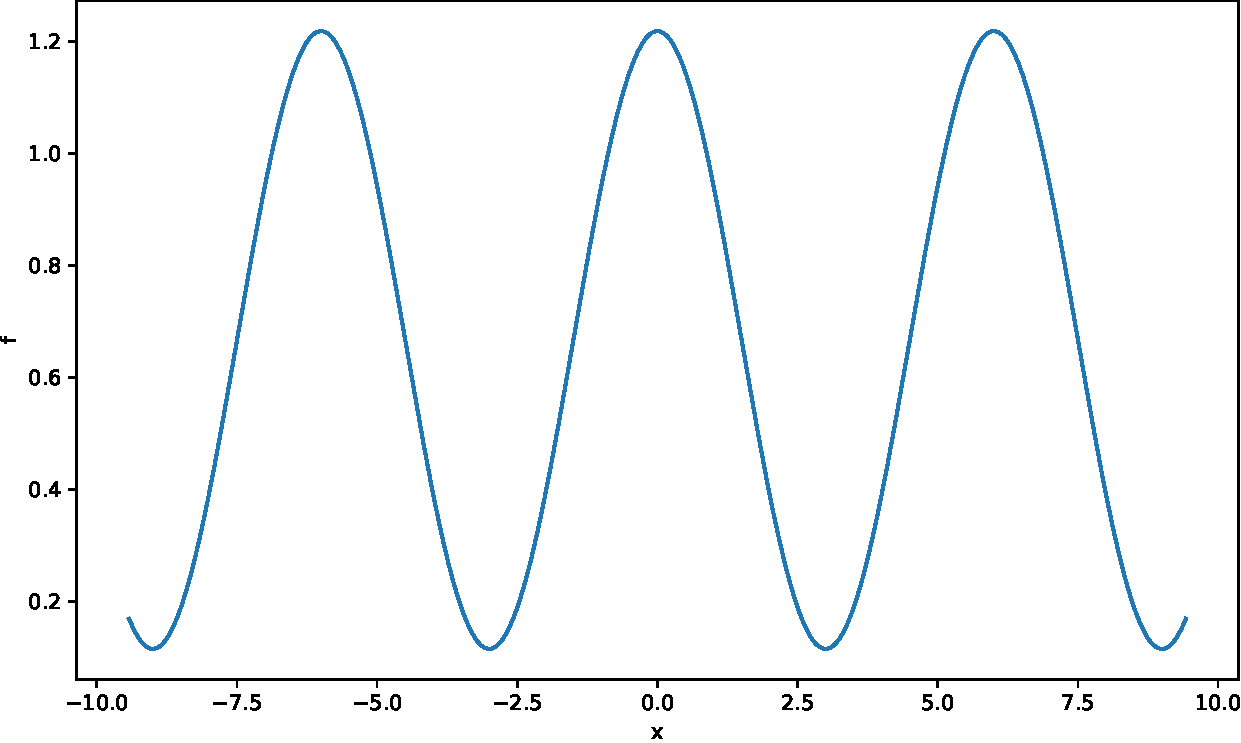
\includegraphics[width=\textwidth]{FourierSeries/Ex1.2.pdf}
		\caption{$N=2$}
	\end{subfigure}
	\hfill
	\begin{subfigure}[b]{0.49\textwidth}
		\centering
		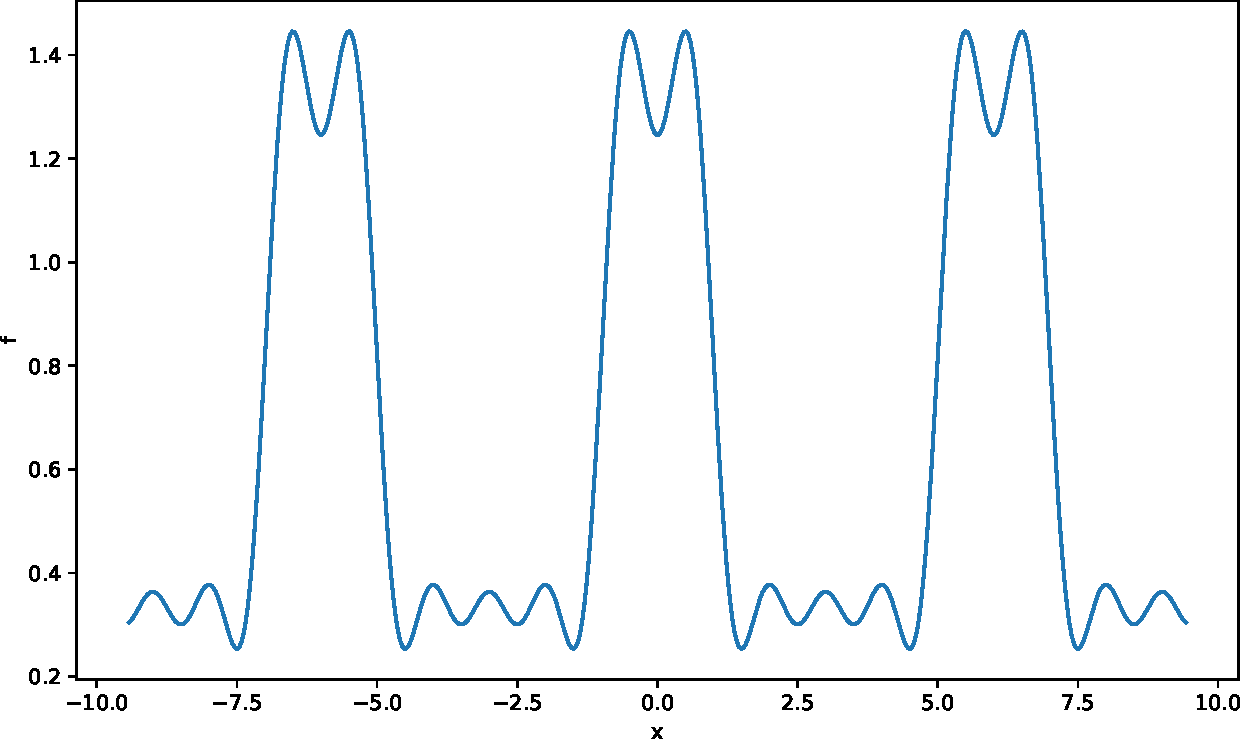
\includegraphics[width=\textwidth]{FourierSeries/Ex1.6.pdf}
		\caption{$N=6$}
	\end{subfigure}
	\\
	\begin{subfigure}[b]{0.49\textwidth}
		\centering
		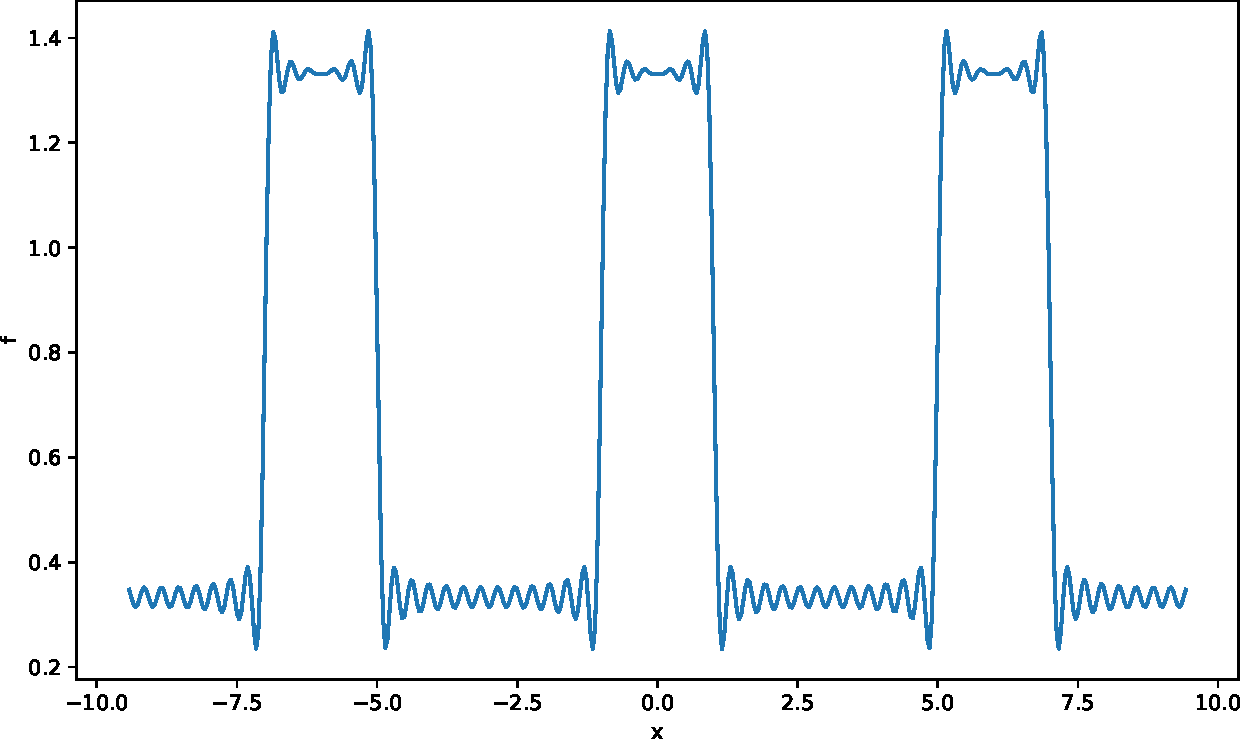
\includegraphics[width=\textwidth]{FourierSeries/Ex1.20.pdf}
		\caption{$N=20$}
	\end{subfigure}
	\hfill
	\begin{subfigure}[b]{0.49\textwidth}
		\centering
		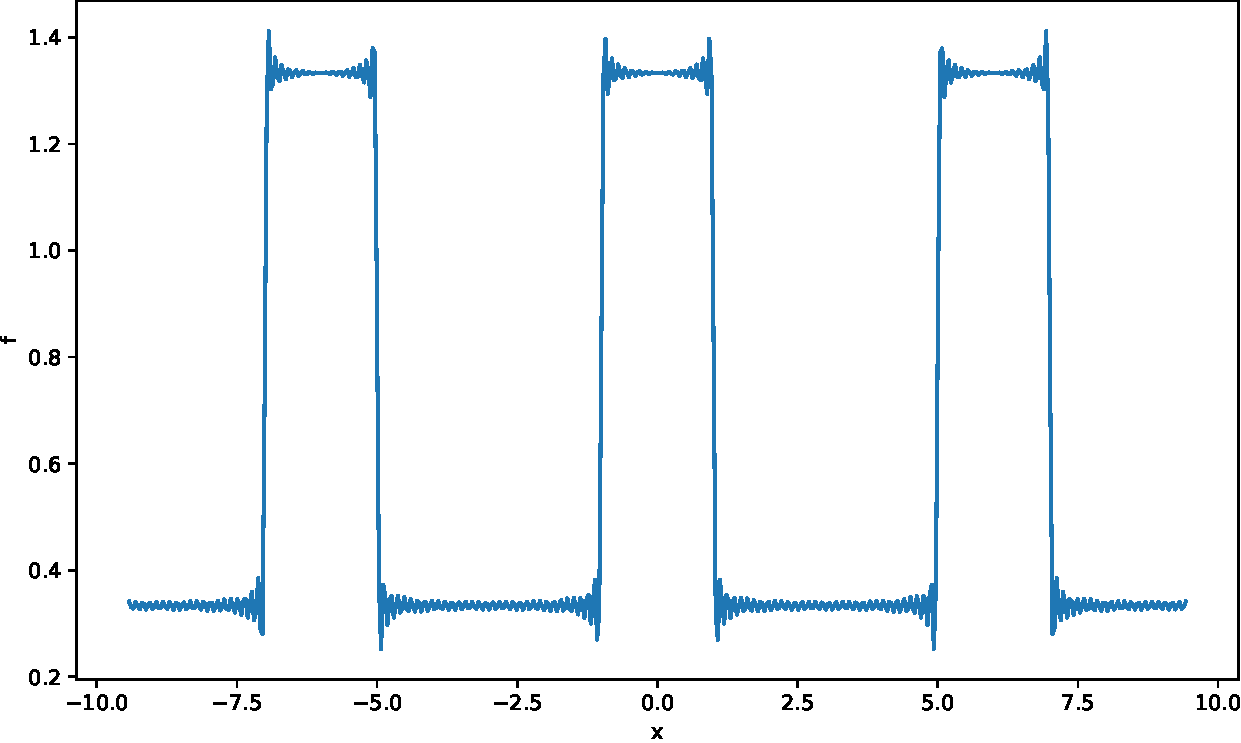
\includegraphics[width=\textwidth]{FourierSeries/Ex1.50.pdf}
		\caption{$N=50$}
	\end{subfigure}
	\caption{Truncated Fourier series from \Cref{eg:fourier1} with various values of $N$.}
	\label{fig:fourieregsub}
\end{figure}

\subsection{Fourier Convergence Theorem}

\begin{definition}
	A function $f$ is piecewise continuous on $[a,b]$ if there exists a finite number of points $a = x_0 < x_1 < \cdots < x_n = b$ such that
	\begin{itemize}
		\item $f$ is continuous on $(x_i, x_{i+1})$,
		\item $\lim_{x \to x_i^{\pm}} f(x) = c_i^{\pm} < \infty$ ($f(x)$ has a finite limit at the endpoints of each subinterval).
	\end{itemize}
\end{definition}

\begin{theorem}[Fourier Convergence Theorem]\label{thrm:fourierconv}
	Assume $f$ and $f'$ are piecewise continuous on $(-L,L)$ and $f(x+2L)=f(x)$. Then the Fourier series
	\[
	\frac{a_0}{2} + \sum_{n=1}^{\infty} \left(a_n \cos{\left(\frac{n\pi x}{L}\right)} + b_n \sin{\left(\frac{n\pi x}{L}\right)}\right)
	\]
	converges to
	\begin{itemize}
		\item $f(x)$ where $f$ is continuous,
		\item $\frac12 \left(\lim_{x\to x_i^-} f(x) + \lim_{x\to x_i^+} f(x)\right)$ where $f$ is discontinuous.
	\end{itemize}
\end{theorem}

\begin{remark}
	Functions like $\frac{1}{x^2}$ and $\log{x}$ have no convergent Fourier series because of the infinite divergences of the function at $x=0$ (so they are not piecewise continuous).
\end{remark}

\begin{remark}
	Functions with an infinite number of discontinuities are not guaranteed to have a convergent Fourier series.
\end{remark}

\begin{eg}[Square wave]\label{eg:squarewave}
	We consider the square wave function
	\[
	f(x) = \begin{cases}0 & \text{if } -L<x<0 \\ L & \text{if } 0<x<L\end{cases}
	\]
	From the Euler-Fourier formulas (\Cref{eq:eulerfourier1,eq:eulerfourier2,eq:eulerfourier3}), we can see that
	\[
	a_0 = \frac{1}{L} \int_{-L}^L f(x) \,dx = \frac{1}{L} \int_0^L L \,dx = L.
	\]
	Next, we find the coefficients $a_n$,
	\begin{align*}
		a_n &= \frac{1}{L} \int_{-L}^L f(x)\cos\left(\frac{n\pi x}{L}\right) dx = \frac{1}{L} \int_0^L L\cos\left(\frac{n\pi x}{L}\right) dx \\
		&= \frac{1}{L} \left[\frac{L^2}{n\pi} \sin\left(\frac{n\pi x}{L}\right)\right]_0^L = 0.
		\intertext{Finally, we find the $b_n$ terms,}
		b_n &= \frac{1}{L} \int_{-L}^L f(x)\sin\left(\frac{n\pi x}{L}\right) dx = \frac{1}{L} \int_0^L \sin\left(\frac{n\pi x}{L}\right) dx \\
		&= -\frac{1}{L} \left[\frac{L}{n\pi} \cos\left(\frac{n\pi x}{L}\right)\right]_0^L = \frac{1}{L} \frac{L^2}{n\pi}(1-\cos(n\pi)) \\
		&= \frac{L}{n\pi}(1-(-1)^n) = \begin{cases}0 & \text{if } n=2m \\ \frac{2L}{(2m+1)\pi} & \text{if } n=2m+1\end{cases}.
	\end{align*}
	Therefore the Fourier series is
	\[
	f(x) = \frac{L}{2} + \frac{2L}{\pi} \sum_{m=0}^{\infty} \frac{1}{2m+1} \sin\left(\frac{(2m+1)\pi x}{L}\right).
	\]
	By the Fourier Convergence Theorem (\Cref{thrm:fourierconv}), the series is convergent at all points where $f$ is continuous (which is everywhere where $x \neq nL$ for $n \in \Z$). At the discontinuities, we will have that the series tends to $\frac{L}{2}$, which is clear in the $x=0$ case as $\sin\left(\frac{(2m+1)\pi x}{L}\right)$ will be zero for all $m$.
\end{eg}

\subsubsection{Errors for Truncated Series}

As we saw in \Cref{fig:fourieregsub}, in practice it is not possible to work with an infinite series, so we must truncate the series taking only the terms up to some finite $N$, i.e. a partial sum:
\[
S_N = \frac{a_0}{2} + \sum_{n=1}^N \left(a_n \cos{\left(\frac{n\pi x}{L}\right)} + b_n \sin{\left(\frac{n\pi x}{L}\right)}\right).
\]
We define the error as
\[
e_N = S_N(x) - f(x),
\]
then we can investigate these in Python. Returning to the square wave from \Cref{eg:squarewave}, we can see that as $N$ increases,
\begin{itemize}
	\item The oscillations near the discontinuities get smaller in amplitude and wavelength.
	\item But the amplitude of the largest oscillation (nearest the discontinuity) does not decrease.
\end{itemize}

This occurrence of the largest oscillation not decreasing in amplitude is called \textbf{Gibbs Phenomenon}. This phenomenon is illustrated in \Cref{fig:gibbs} for the series in \Cref{eg:squarewave} with $L=1$.

\begin{figure}[!ht]
	\centering
	\begin{subfigure}[b]{0.49\textwidth}
		\centering
		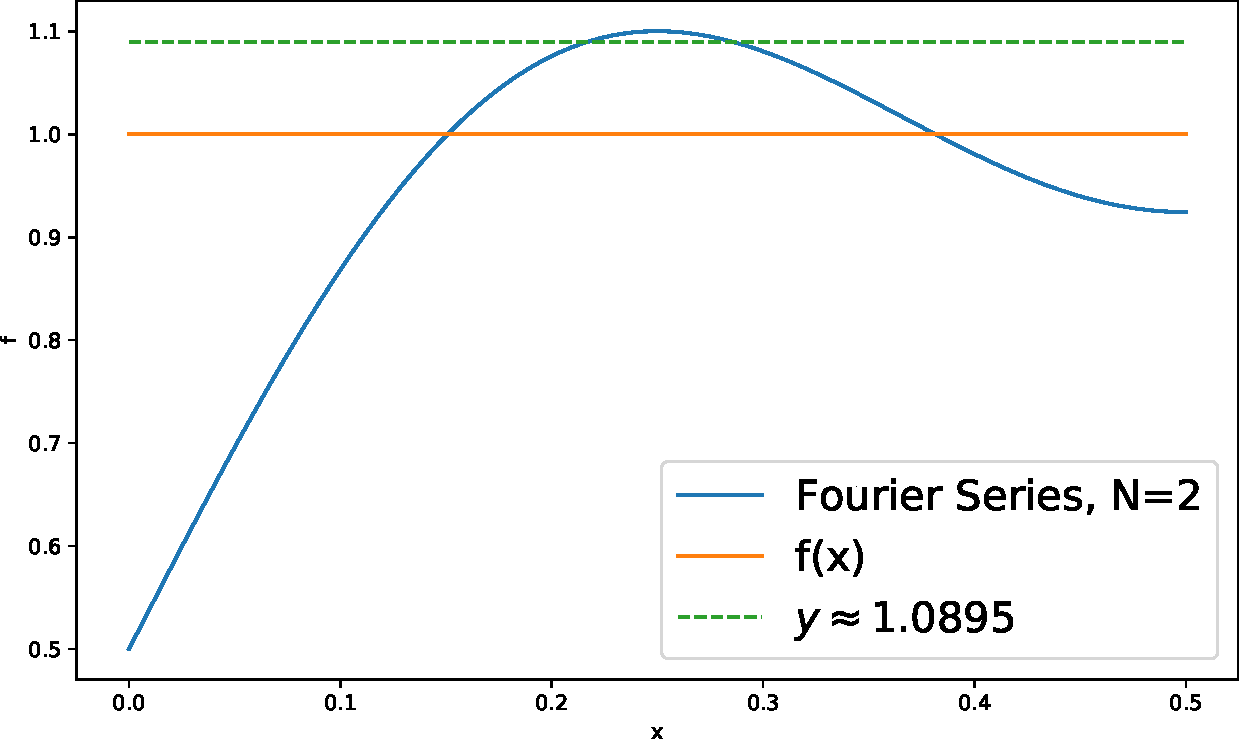
\includegraphics[width=\textwidth]{FourierSeries/Gibbs2.pdf}
		\caption{$N=2$}
	\end{subfigure}
	\hfill
	\begin{subfigure}[b]{0.49\textwidth}
		\centering
		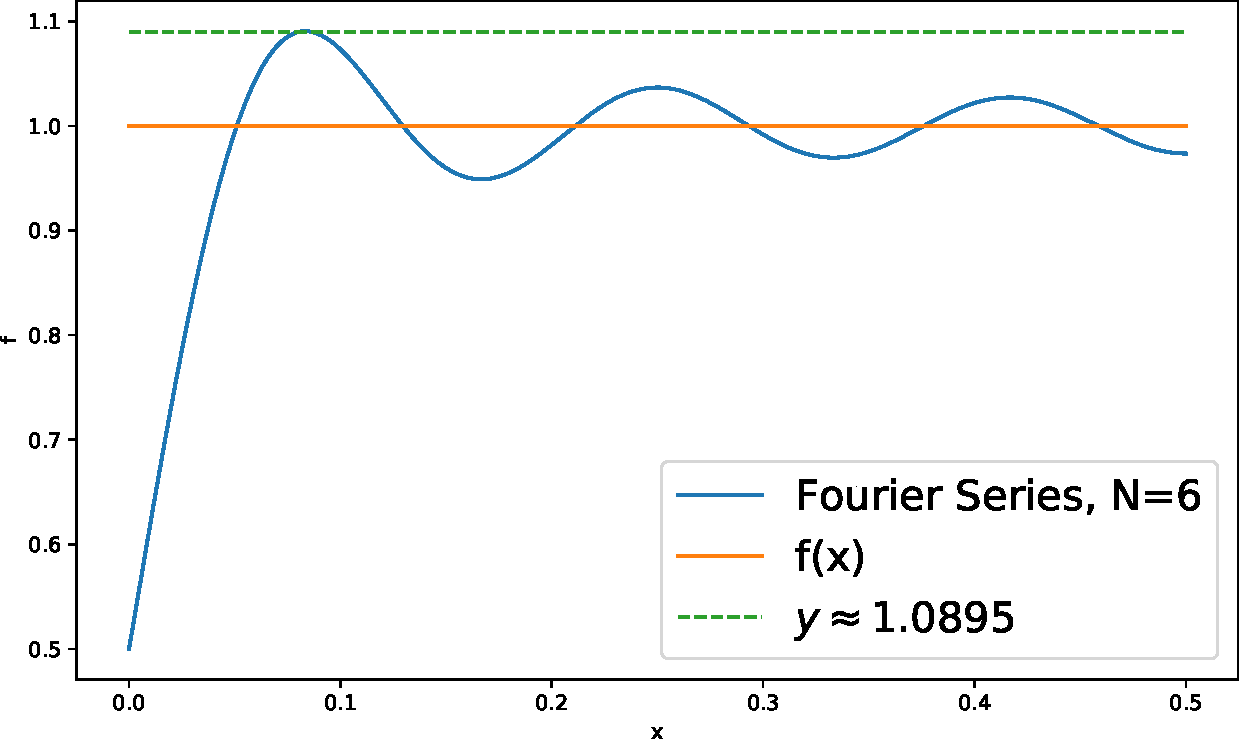
\includegraphics[width=\textwidth]{FourierSeries/Gibbs6.pdf}
		\caption{$N=6$}
	\end{subfigure}
	\\
	\begin{subfigure}[b]{0.49\textwidth}
		\centering
		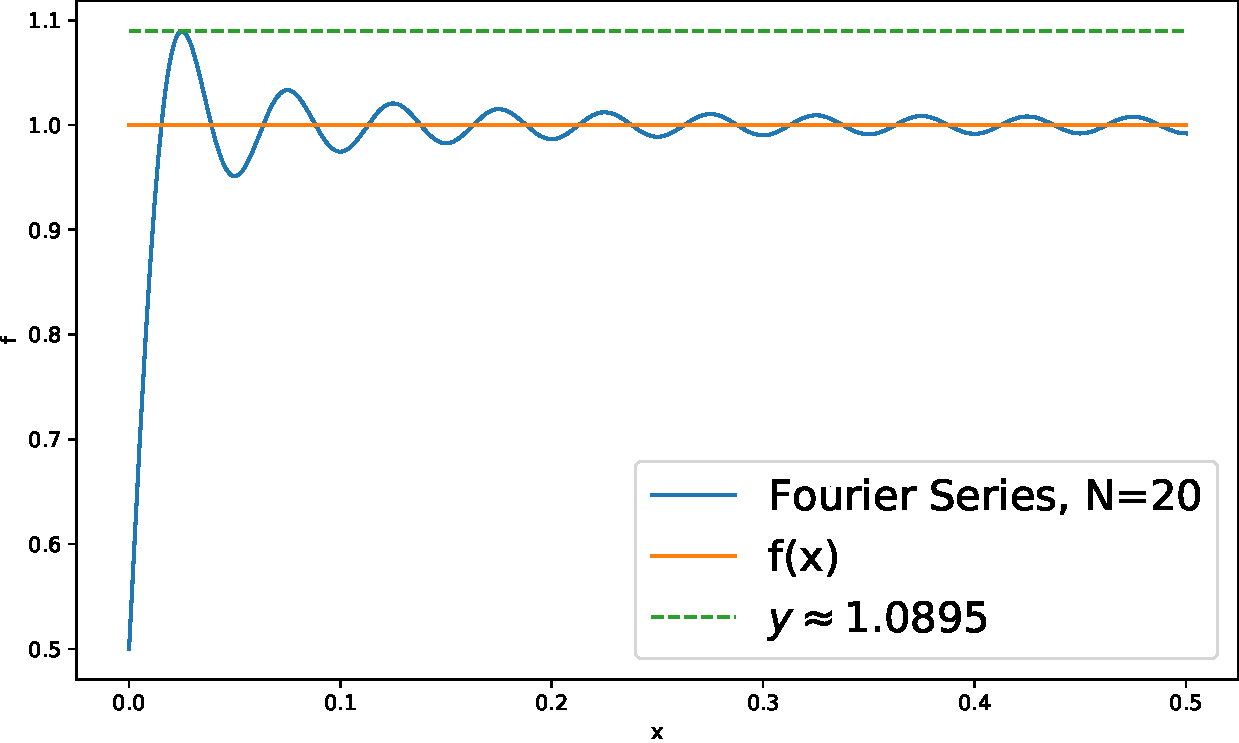
\includegraphics[width=\textwidth]{FourierSeries/Gibbs20.pdf}
		\caption{$N=20$}
	\end{subfigure}
	\hfill
	\begin{subfigure}[b]{0.49\textwidth}
		\centering
		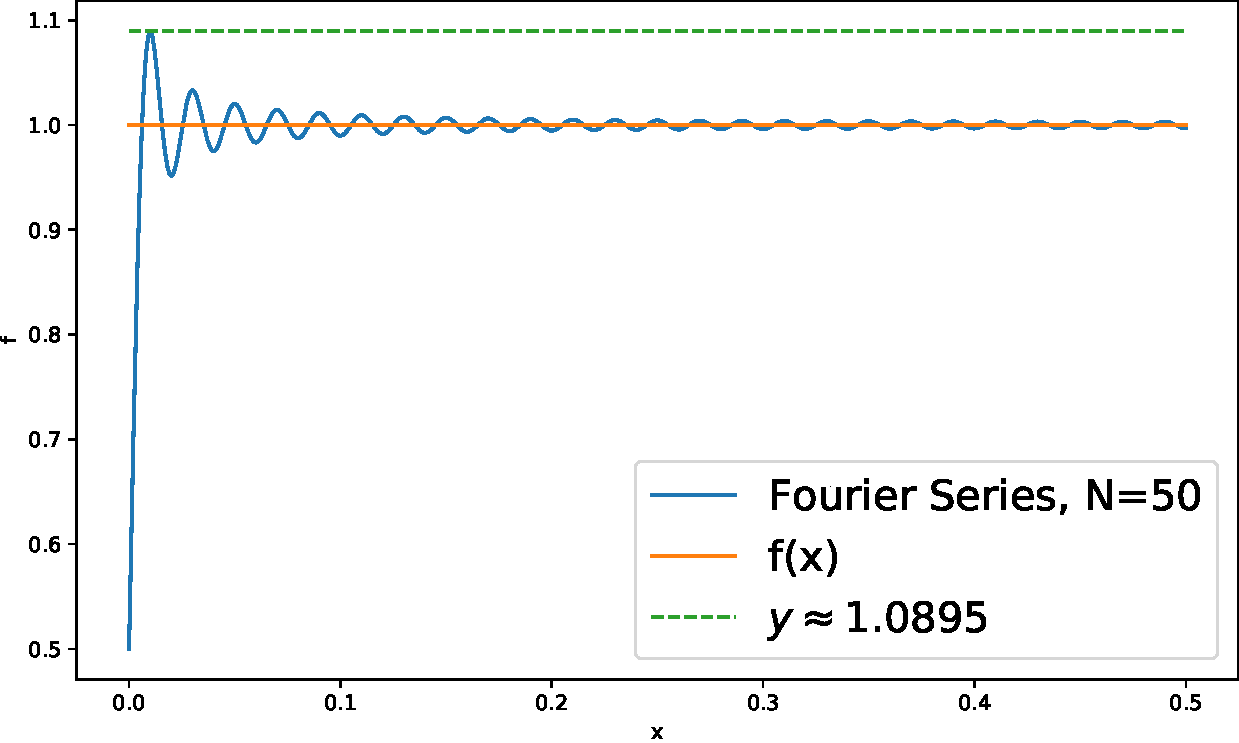
\includegraphics[width=\textwidth]{FourierSeries/Gibbs50.pdf}
		\caption{$N=50$}
	\end{subfigure}
	\caption{For the Fourier series from the square wave example with $L=1$, we observe that the maximum amplitude of the error around $x=0$ does not decrease as $N$ increases. Instead, it tends to a value of approximately 0.0895.\protect\footnotemark}
	\label{fig:gibbs}
\end{figure}

\footnotetext{In fact, we can calculate the error to be \[\frac{1}{\pi} \int_0^{\pi}\frac{\sin t}{t}dt - \frac12 = 0.089489877236\ldots \tag{\href{https://oeis.org/A243268}{OEIS A243268}}\] For a full derivation of this result, see \href{https://en.wikipedia.org/wiki/Gibbs_phenomenon}{Wikipedia}.}

\subsection{Other Results on Fourier Series}

\subsubsection{Complex Form}\label{sec:fouriercomplex}

Now we will see that we can write the Fourier series in \Cref{def:fourier} in terms of complex exponentials instead of trigonometric functions. This will make use of the fact that
\[
\cos(x) = \frac{e^{ix} + e^{-ix}}{2} \quad \text{and} \quad \sin(x) = \frac{e^{ix} - e^{-ix}}{2i}.
\]

For simplicity in the following derivation, we shall denote the argument of the trig functions by $k = \frac{n\pi x}{L}$.

\begin{align*}
	f(x) &= \frac{a_0}{2} + \sum_{n=1}^{\infty} \left(a_n \cos{\left(\frac{n\pi x}{L}\right)} + b_n \sin{\left(\frac{n\pi x}{L}\right)}\right) \\
	&= \frac{a_0}{2} + \sum_{n=1}^{\infty} \left(a_n \frac{e^{ik} + e^{-ik}}{2} + b_n \frac{e^{ik} - e^{-ik}}{2i}\right) \\
	&= \frac{a_0}{2} + \sum_{n=1}^{\infty} \frac{a_n - ib_n}{2} e^{ik} + \sum_{n=1}^{\infty} \frac{a_n + ib_n}{2} e^{-ik} \\
	&= \sum_{n=-\infty}^{\infty} c_n e^{in\pi x/L},
\end{align*}
where
\[
c_0 = \frac{a_0}{2}, \quad c_n = \frac{a_n - ib_n}{2}, n>0 \quad c_n = \frac{a_n + ib_n}{2}, n<0.
\]
Thus, we have formulas to convert real coefficients into complex coefficients. In addition, to convert complex coefficients into real coefficients, we can use the following formulas
\[
a_0 = 2c_0, \quad a_n = c_n + c_{-n}, \quad b_n = i(c_n - c_{-n}).
\]

To compute complex coefficients directly, we can use the Euler-Fourier formulas (\Cref{eq:eulerfourier1,eq:eulerfourier2,eq:eulerfourier3}), we find that
\begin{equation}\label{eq:fouriercomplexcoeffs}
	c_n = \frac{1}{2L} \int_{-L}^L f(x) e^{-in\pi x/L} \,dx.
\end{equation}

An alternative derivation of this formula for the $c_n$ terms is as follows: We have that
\[
f(x) = \sum_{n=-\infty}^{\infty} c_n e^{in\pi x/L}.
\]
We define a slightly different inner product from the one for real functions in \Cref{eq:innerprod}:
\begin{equation}\label{eq:innerprodcomplex}
	\left(u(x), v(x)\right) = \int_{-L}^L u(x)v^*(x) \,dx,
\end{equation}
where $v^*(x)$ is the complex conjugate of $v(x)$. From this definition, observe that
\[
\left(e^{in\pi x/L}, e^{im\pi x/L}\right) = 2L\delta_{mn},
\]
which we find using the new definition of the inner product,
\begin{align*}
	\left(e^{in\pi x/L}, e^{im\pi x/L}\right) &= \int_{-L}^L e^{in\pi x/L}e^{-im\pi x/L} \,dx \tag{$n \neq m$} \\
	&= \left[ \frac{Le^{i(n-m)\pi x/L}}{i(n-m)\pi} \right]_{-L}^L \\
	&= \frac{L}{i(n-m)\pi} \left(e^{ik\pi} - e^{-ik\pi}\right) \tag{$k=n-m$} \\
	&= \cos(k\pi) + i\sin(k\pi) - \cos(-k\pi) - i\sin(-k\pi) = 0.
\end{align*}
And for $n=m$,
\begin{align*}
	(e^{in\pi x/L}, e^{in\pi x/L}) &= \int_{-L}^L e^{in\pi x/L}e^{-in\pi x/L} \,dx \\
	&= \int_{-L}^L dx = 2L.
\end{align*}
Therefore the functions $e^{in\pi x/L}$ are orthogonal for all $n$, hence they form a basis. Finally, we can find the formula for $c_n$:
\begin{align*}
	\left(f(x), e^{im\pi x/L}\right) &= \sum_n c_n \cancelto{2L\delta_{mn}}{(e^{in\pi x/L}, e^{im\pi x/L})} = 2L c_m \\
	\implies c_m &= \frac{1}{2L} \int_{-L}^L f(x) e^{-im\pi x/L} \,dx.
\end{align*}

\begin{remark}
	While we now have the option to expand functions either in terms of $\sin$ and $\cos$ or complex exponentials, in practice it is usually easier to use the trig functions for real functions and exponentials for complex functions.
\end{remark}

\begin{eg}
	Using complex form, find the Fourier series of the function
	\[
	f(x) = \text{sgn}\,x = \begin{cases} -1 & \text{if } -\pi \leq x \leq 0 \\ 1 & \text{if } 0 < x \leq \pi \end{cases}.
	\]
	Calculating the coefficient $c_0$:
	\[
	c_0 = \frac{1}{2\pi} \int_{-\pi}^{\pi} f(x) \,dx = 0,
	\]
	since $f$ is an odd function. Next, we find the coefficients $c_n$:
	\begin{align*}
		c_n &= \frac{1}{2\pi} \int_{-\pi}^{\pi} f(x){e^{-inx}}dx \\
		&= \frac{1}{2\pi}\left[ \int_{-\pi}^0 \left( {-1} \right){e^{-inx}}dx + \int_0^{\pi} e^{-inx}dx \right] \\
		&= \frac{1}{2\pi} \begin{bmatrix} -\dfrac{\left. \left( e^{-inx} \right) \right|_{-\pi }^0}{-in} + \dfrac{\left. \left( e^{-inx} \right) \right|_0^\pi }{-in} \end{bmatrix} \\
		&= \frac{i}{2\pi n}\left[-\left(1-e^{in\pi} \right) + e^{-in\pi}-1 \right] \\
		&= \frac{i}{2\pi n}\left[e^{in\pi} + e^{-in\pi}-2 \right] = \frac{i}{\pi n} \begin{bmatrix} \dfrac{e^{in\pi} + e^{-in\pi}}{2}-1 \end{bmatrix} \\
		&= \frac{i}{\pi n}\left[\cos(n\pi)-1\right] = \frac{i}{\pi n}\left[(-1)^n-1\right].
	\end{align*}
	If $n=2k$, we have that $c_n = 0$, and if $n=2k-1$, $c_n = -\frac{2i}{(2k-1)\pi}$. Hence, we can write the Fourier series in complex form as
	\[
	f(x) = -\frac{2i}{\pi} \sum_{k=-\infty}^{\infty} \frac{1}{2k-1}e^{i(2k-1)x}.
	\]
\end{eg}

\subsubsection{Even and Odd Functions}\label{sec:evenoddfourier}

Recall the definitions of even and odd functions:
\begin{itemize}
	\item Even function: $f(x) = f(-x)$.
	\item Odd function: $f(x) = -f(-x)$.
\end{itemize}

First, we calculate the Fourier coefficients where $f$ is an even function:
\begin{align*}
	a_n &= \frac{1}{L} \int_{-L}^L f(x)\cos\left(\frac{n\pi x}{L}\right) dx \\
	&= \frac{1}{L} \left(\int_{-L}^0 f(x)\cos\left(\frac{n\pi x}{L}\right) dx + \int_0^L f(x)\cos\left(\frac{n\pi x}{L}\right) dx\right) \\
	&= \frac{2}{L} \int_0^L f(x)\cos\left(\frac{n\pi x}{L}\right) dx,
\end{align*}
since $f(x)\cos\left(\frac{n\pi x}{L}\right)$ is an even function, and
\[
b_n = \frac{1}{L} \int_{-L}^L f(x)\sin\left(\frac{n\pi x}{L}\right) = 0,
\]
since the integrand $f(x)\sin\left(\frac{n\pi x}{L}\right)$ is an odd function and the limits of integration are symmetric.

Similarly, the Fourier coefficients for an odd function are found to be
\[
a_n = 0 \quad b_n = \frac{2}{L} \int_0^L f(x)\sin\left(\frac{n\pi x}{L}\right) dx.
\]

Therefore, the Fourier series for an odd function will only be in terms of sines, and the series for an even function will contain only cosines.

\begin{eg}[Sawtooth Function]\label{eg:sawtooth}
	The sawtooth function is given by $f(x)=x$ for $-L\leq x<L$, with $f(x+2L) = f(x)$.
	
	Therefore, we have that $f$ is an odd function, therefore $a_n = 0$ for all $n$.
	
	Next, we find the $b_n$s using integration by parts
	\begin{align*}
		b_n &= \frac{2}{L} \int_0^L f(x)\sin\left(\frac{n\pi x}{L}\right) dx \\
		&= \frac{2}{L} \int_0^L x\sin\left(\frac{n\pi x}{L}\right) dx \\
		&= \frac{2}{L} \left(\left[ -\frac{xL}{n\pi}\cos\left(\frac{n\pi x}{L}\right) \right]_0^L + \frac{L}{n\pi}\cancelto{0}{\int_0^L \cos\left(\frac{n\pi x}{L}\right) dx} \right) \\
		&= -\frac{2}{L} \frac{L^2 (-1)^n}{n\pi} \tag{Since $\cos(n\pi) = (-1)^n$} \\
		&= \frac{2L}{n\pi}(-1)^{n+1}.
	\end{align*}
	Therefore the resulting Fourier series is
	\[
	f(x) = \frac{2L}{\pi} \sum_{n=1}^{\infty} \frac{(-1)^{n+1}}{n} \sin\left(\frac{n\pi x}{L}\right).
	\]
	The truncated Fourier series with the first 20 terms is shown in \Cref{fig:fouriersawtooth}.
\end{eg}

\begin{figure}[!ht]
	\centering
	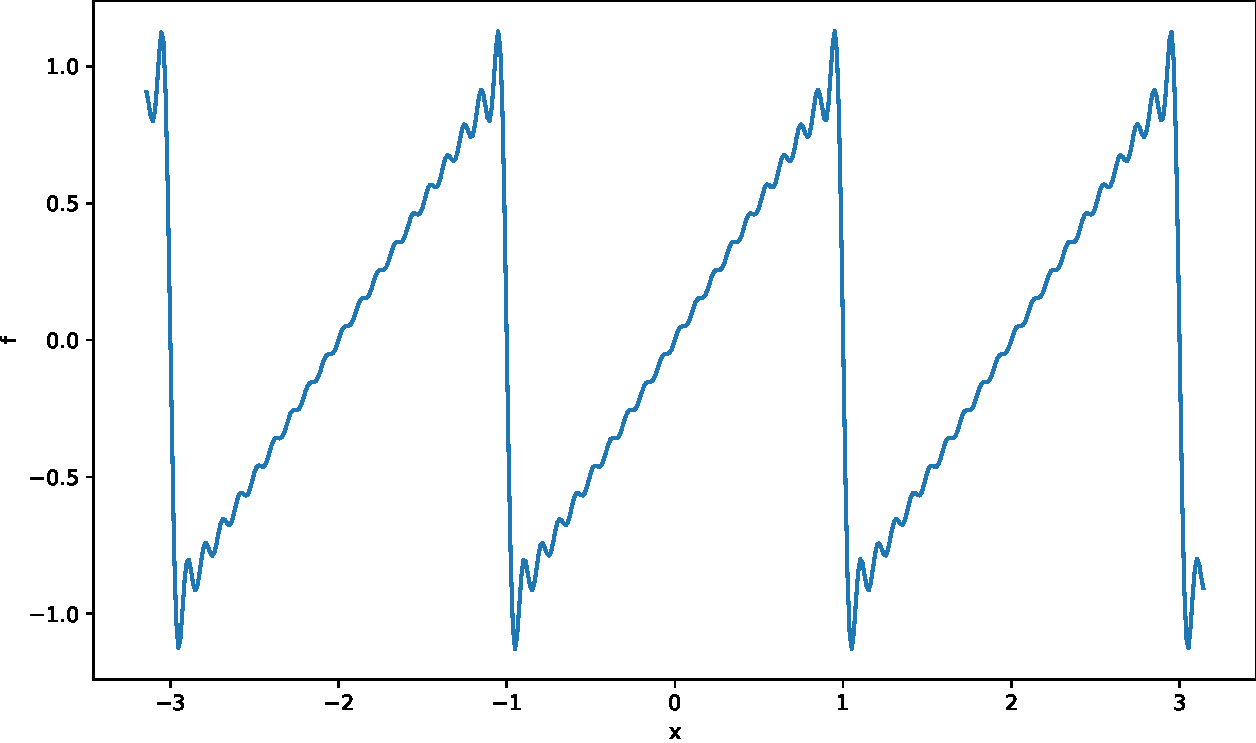
\includegraphics[width=0.7\textwidth]{FourierSeries/Sawtooth20.pdf}
	\caption{Fourier series for the sawtooth function in \Cref{eg:sawtooth} with first 20 terms.}
	\label{fig:fouriersawtooth}
\end{figure}

Note that we can still apply these formulas in the case where we have functions that are only defined on the interval $(0,L)$ by extending the function onto the interval $(-L,0)$ (then the periodicity condition $f(x+2L)=f(x)$ can be used to extend to the rest of the real line). The natural ways of doing this extension are the even extension and the odd extension, as in \Cref{fig:evenoddextension}.

\begin{figure}[!ht]
	\centering
	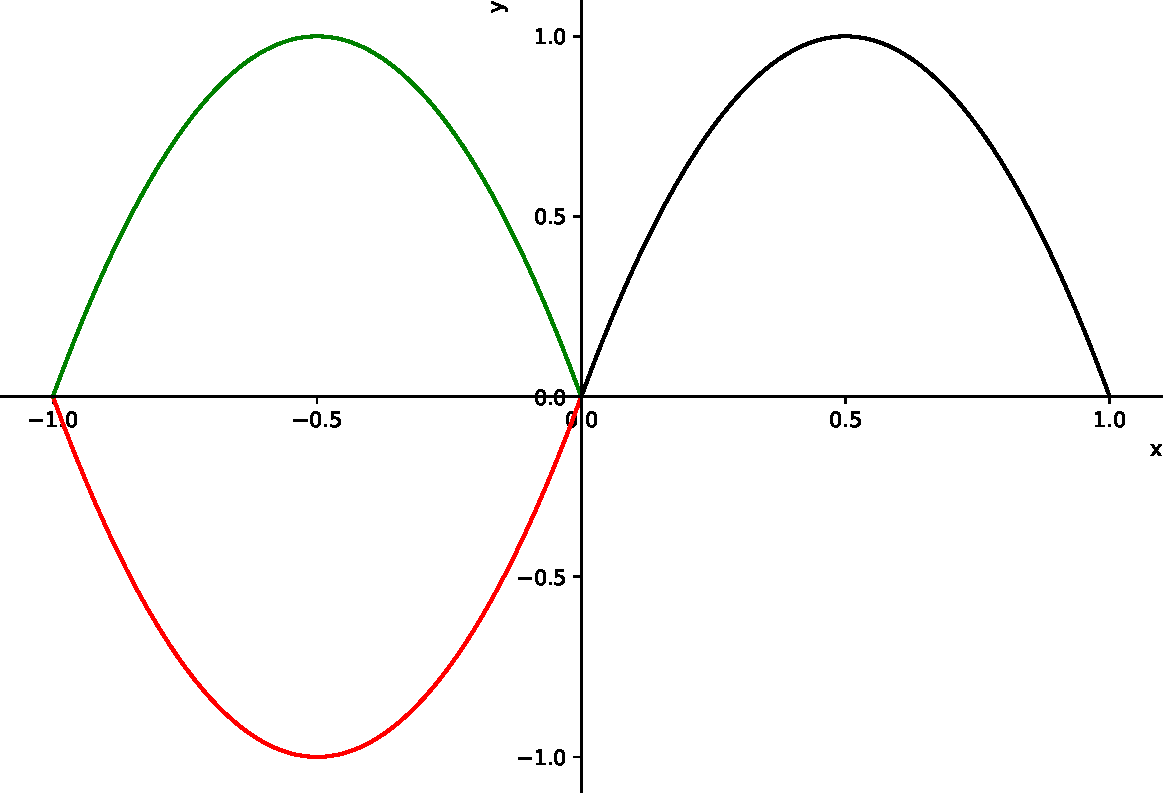
\includegraphics[width=0.6\textwidth]{EvenOddExtension.pdf}
	\caption{The function $f(x) = 4x(1-x)$ (black), with its even (green) and odd (red) extensions.}
	\label{fig:evenoddextension}
\end{figure}

Algebraically, given some function $f(x)$ for $x \in [0,L]$,
\begin{itemize}
	\item Its even extension can be defined as
	\[
		h(x) = \begin{cases}
			f(x) & x \in [0,L] \\
			f(-x) & x \in [-L,0]
		\end{cases}
	\]
	This will have a cosine series.
	\item Its odd extension can be defined as
	\[
	h(x) = \begin{cases}
		f(x) & x \in (0,L) \\
		0 & x = -L,0,L \\
		f(-x) & x \in (-L,0)
	\end{cases}
	\]
	This will have a sine series.
\end{itemize}

\subsubsection{Parseval's Theorem}

\begin{theorem}[Parseval's Theorem]\label{thrm:parseval}
	Suppose $f$ is a square integrable function on $[-L,L]$ (i.e. $f$ and $f^2$ are integrable on this interval) with the Fourier series
	\[
	f(x) = \frac{a_0}{2} + \sum_{n=1}^{\infty} \left(a_n \cos{\left(\frac{n\pi x}{L}\right)} + b_n \sin{\left(\frac{n\pi x}{L}\right)}\right)
	\]
	Then
	\[
	\lVert f\rVert^2 = (f,f) = \int_{-L}^L f^2(x) \,dx = 2L\sum_{n=-\infty}^{\infty} |c_n|^2 = L\left(\frac{a_0^2}{2} + \sum_{n=1}^{\infty}(a_n^2 + b_n^2)\right).
	\]
\end{theorem}

\begin{proof}
	We prove this theorem using the complex form of the Fourier series, as introduced in \Cref{sec:fouriercomplex}.
	\begin{align*}
		\lVert f\rVert^2 = (f,f) &= \left(\sum_n c_n e^{in\pi x/L}, \sum_m c_m e^{im\pi x/L}\right) \\
		&= \sum_n \sum_m c_n c_m^* \cancelto{2L\delta_{mn}}{(e^{in\pi x/L}, e^{im\pi x/L})} \\
		&= \sum_n c_n c_m^* 2L = 2L \sum_n |c_n|^2.
	\end{align*}
	Applying the relationships between $a_n$, $b_n$, and $c_n$ in \Cref{eq:fouriercomplexcoeffs}, we have that, for $n\neq0$,
	\[
	|c_n|^2 = \left|\frac{a_n \mp ib_n}{2}\right|^2 = \left(\frac{a_n}{2}\right)^2 + \left(\frac{b_n}{2}\right)^2 = \frac14(a_n^2 + b_n^2)
	\]
	So
	\begin{align*}
		2L\sum_{n=-\infty}^{\infty} |c_n|^2 &= 2L\left( |c_0|^2 + \sum_{n=-\infty}^{-1} |c_n|^2 + \sum_{n=1}^{\infty} |c_n|^2 \right) \\
		&= 2L\left( \left(\frac{a_0}{2}\right)^2 + \sum_{n=-\infty}^{-1} \frac14(a_n^2 + b_n^2) + \sum_{n=1}^{\infty} \frac14(a_n^2 + b_n^2)\right) \\
		&= 2L\left(\frac{a_0^2}{4} + 2\sum_{n=1}^{\infty} \frac14(a_n^2 + b_n^2)\right) \\
		&= L\left(\frac{a_0^2}{2} + \sum_{n=1}^{\infty}(a_n^2 + b_n^2)\right).
	\end{align*}
\end{proof}

\begin{eg}
	We apply Parseval's Theorem to the sawtooth function in \Cref{eg:sawtooth}. Recall that we had the function $f(x) = x$ for $-L\leq x < L$, with corresponding Fourier series
	\[
	f(x) = \frac{2L}{\pi} \sum_{n=1}^{\infty} \frac{(-1)^{n+1}}{n} \sin\left(\frac{n\pi x}{L}\right).
	\]
	Then
	\[
	\lVert f \rVert^2 = (f,f) = \int_{-L}^L x^2 \,dx = \frac{2L^3}{3}
	\]
	by direct calculation. Now, applying Parseval's Theorem,
	\begin{align*}
		\frac{2L^3}{3} &= \int_{-L}^L f^2(x) \,dx = L \sum_{n=1}^{\infty} b_n^2 \\
		&= L \sum_{n=1}^{\infty} \frac{4L^2}{\pi^2} \frac{1}{n^2} \\
		\implies \frac{4L^3}{\pi^2} \sum_{n=1}^{\infty} \frac{1}{n^2} &= \frac{2L^3}{3} \\
		\implies \sum_{n=1}^{\infty} \frac{1}{n^2} &= \frac{\pi^2}{6}.
	\end{align*}
	This rather beautiful formula for the sum of the reciprocals of the square numbers was proved by Euler (though using a different method) and was known as the \href{https://en.wikipedia.org/wiki/Basel_problem}{Basel problem}.
\end{eg}